
\documentclass{beamer}
\usepackage{ucs}
\usepackage[utf8x]{inputenc}
\usepackage[T1]{fontenc}

\usepackage{graphicx}
\usepackage{tipa}

\begin{document}
\title{Constraint Grammar in Dialogue Systems}   
\author{Lene Antonsen, Saara Huhmarniemi, Trond Trosterud \\
Centre for Sámi Language Technology \begin{figure}  \scalebox{0.10}[0.10]{
\includegraphics{img/LogoEngelsk}} \end{figure} 
}
\date


\frame{\titlepage} 

\frame{\frametitle{Contents}\tableofcontents} 


\section{1. Introduction} 

\frame{\frametitle{Parser-based CALL programs}
Parser-based CALL programs for learners of North Sámi based on pre-existing LT resources developed at the University of Tromsø:
\begin{itemize}
\item finite state morphological analyser/generator (fst)
\item constraint grammar (CG) parser
\item number word generator (xfst)
\end{itemize} 

\vspace{0.5cm}
The morphological analyser/generator is implemented with fst and compiled with the Xerox compilers twolc and lexc. \\
The morphological disambiguator is implemented in the CG-framework.
}

\frame{\frametitle{North Sámi VISL} 
\scalebox{0.24}[0.24]{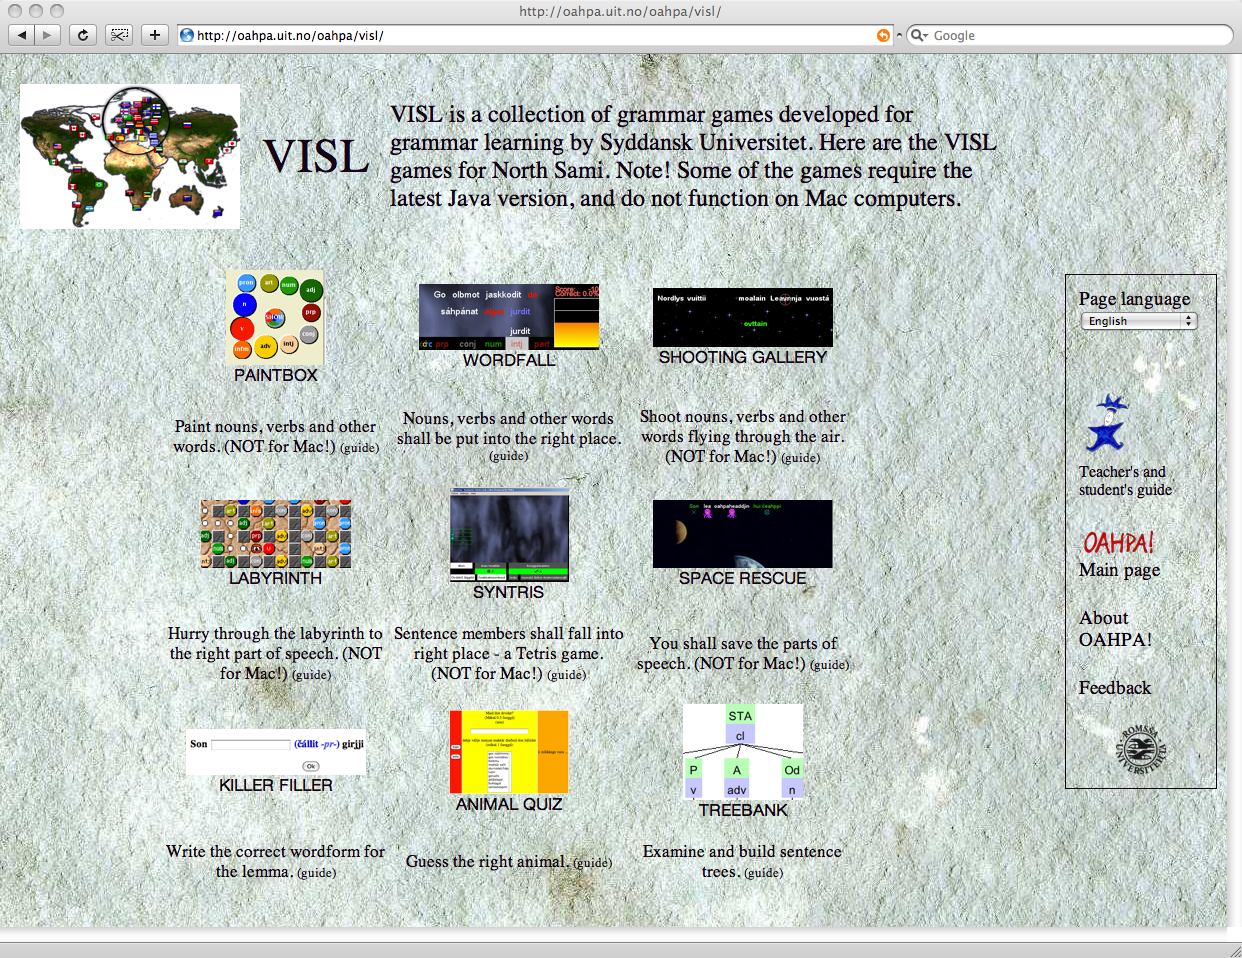
\includegraphics{img/oahpavisl.png}} \\
}


\frame{\frametitle{http://oahpa.uit.no/} 
\scalebox{0.30}[0.30]{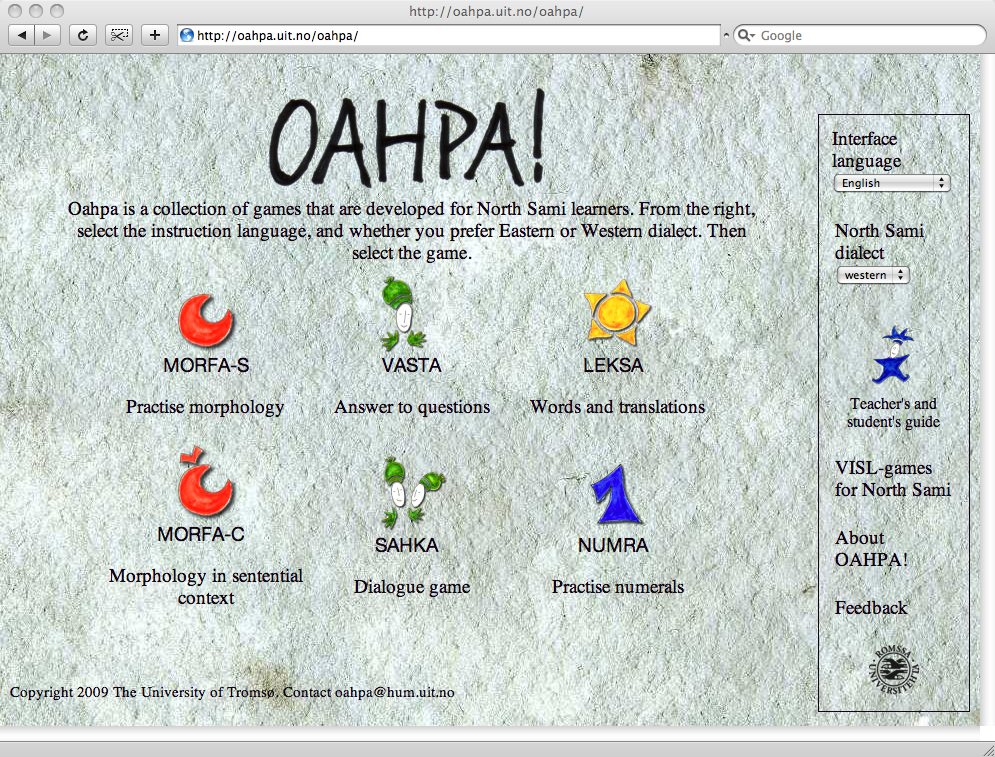
\includegraphics{img/Oahpanew.png}} \\
}


\section{2. Analysing the user's input}

\frame{\frametitle{Pedagogical lexicon} 
\scalebox{0.40}[0.40]{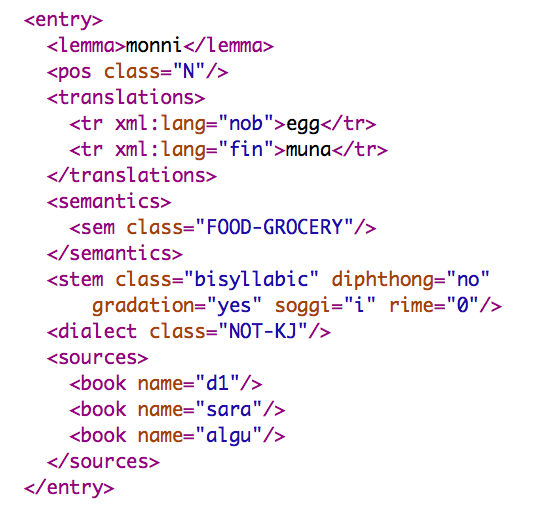
\includegraphics{img/nounlexiconMonni.png}} \\
}



\frame{\frametitle{Sentence generator} 
used in \textbf{Vasta} -- the question-answer drill and in \textbf{Morfa-C} -- morphological exercises in a sentential frame \\
\vspace{0.5cm}
\scalebox{0.50}[0.50]{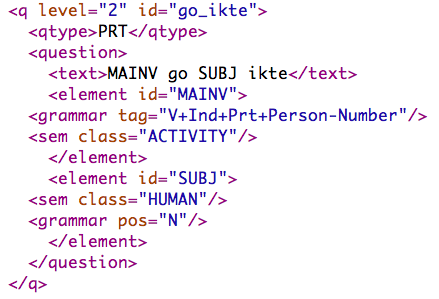
\includegraphics{img/sentencegenerator.png}} \\
\vspace{0.5cm}
(MAINV question-particle SUBJ yesterday)
}

\frame{\frametitle{Sentence generator in Vasta} 
\scalebox{0.50}[0.50]{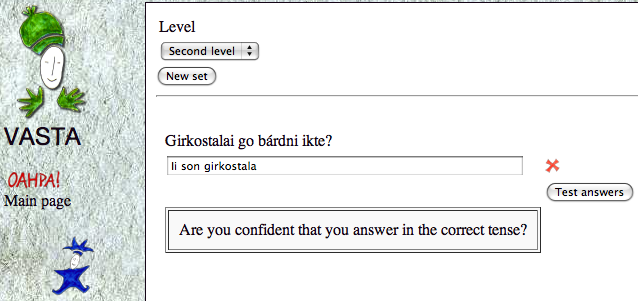
\includegraphics{img/Vasta_sentencegen_example.png}} \\
\vspace{0.5cm}
("Did the boy go to church yesterday?" \\
"No, he does not.")
}

\frame{\frametitle{Constraint Grammar parser -- vislcg3}
CG is robust enough for handling unconstrained input, and at the same time accurate enough to identify errors. \\
}


\frame{\frametitle{Sahka -- the dialogue program} 
\scalebox{0.39}[0.41]{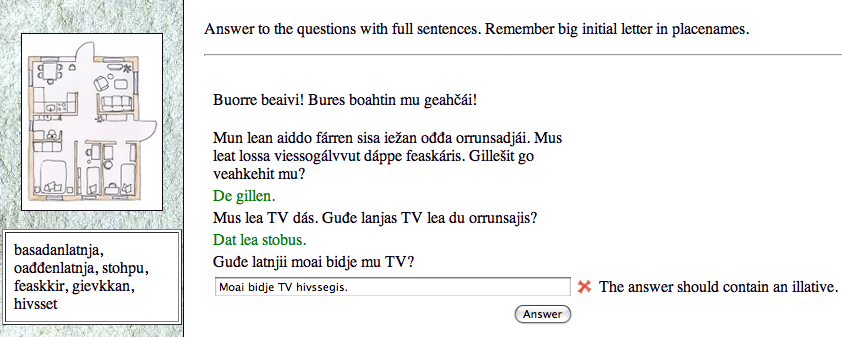
\includegraphics{img/TVhivssegis.png}} \\ \pause
\vspace{0.5cm}
Question: "In which room should we place the TV?" \\
Answer: "We should place it in the toilet."
}


\frame{\frametitle{Schematical view of the process} 
\scalebox{0.55}[0.55]{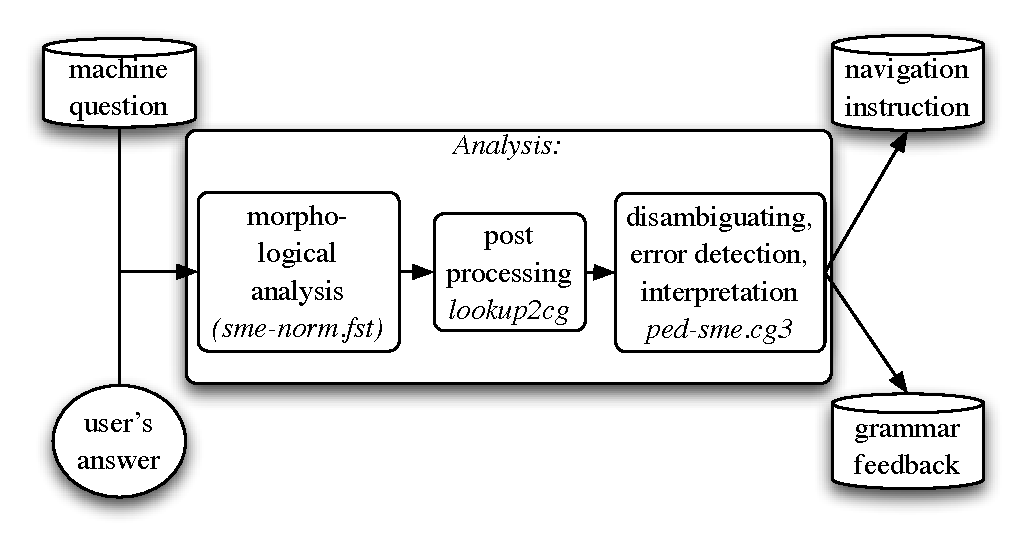
\includegraphics{img/qa2.pdf}} \\
}


%\frame{\frametitle{Morphological analysis} 
%\scalebox{0.35}[0.35]{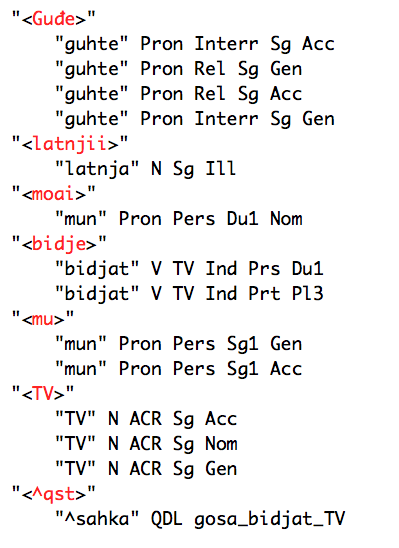
\includegraphics{img/GudelatnjiiQ.png}{img/GudelatnjiiB.png}}\scalebox{0.35}[0.35]{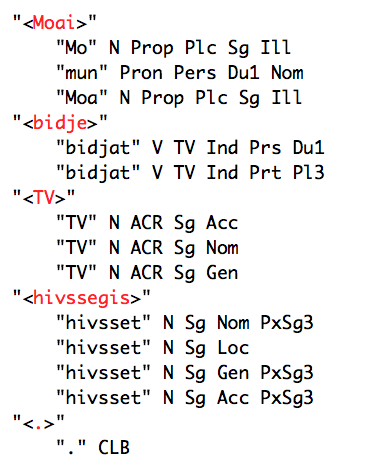
\includegraphics{img/GudelatnjiiA.png}{img/GudelatnjiiB.png}} \\
%}

\section{3. Navigation and collecting information}


\frame{\frametitle{Target tag} 
What do you want to drink?\\
\vspace{0.5cm}
\scalebox{0.4}[0.4]{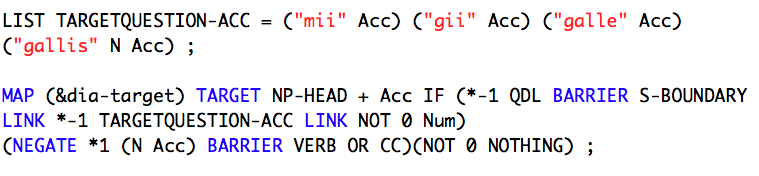
\includegraphics{img/target_acc.png}} \\
}


\frame{\frametitle{Assignment of navigation tag} 
\scalebox{0.37}[0.37]{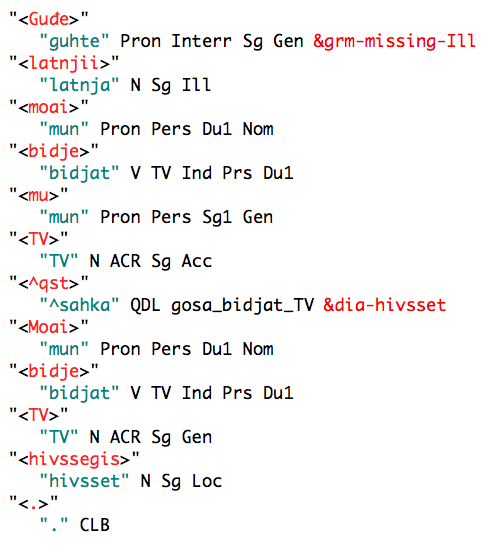
\includegraphics{img/hivssegisCGanal.png}} \\
\scalebox{0.35}[0.35]{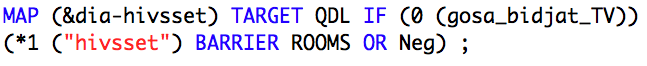
\includegraphics{img/hivsset_tag.png}} \\
}

\frame{\frametitle{Tags for postive and negative answer} 
Do you have children? \\ What do you want to drink?\\
\vspace{0.5cm}
\scalebox{0.5}[0.5]{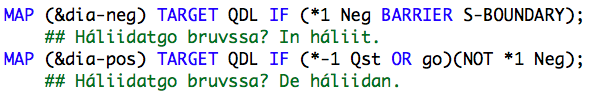
\includegraphics{img/aff_or_neg_colours.png}} \\
}

\frame{\frametitle{Tag for jumping over the next question} 
Do you have children? How many children do you have?\\
Do you work? What kind of work do you have?\\
Do you have a car? What kind of car do you have?\\
\vspace{0.5cm}
\scalebox{0.55}[0.55]{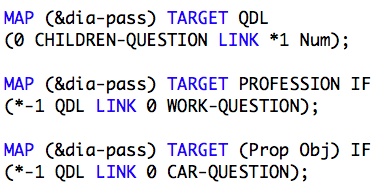
\includegraphics{img/pass_rules.png}} \\
}


\frame{\frametitle{Collecting information from the input} 
What is your name?\\ What car do you have? \\ Where do you live? \\
\vspace{0.5cm}
\scalebox{0.45}[0.45]{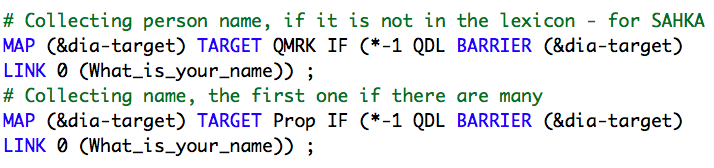
\includegraphics{img/picking_name_new.png}} \\
}


\frame{\frametitle{Navigating in the dialogue -- alternative links} 
\scalebox{0.35}[0.35]{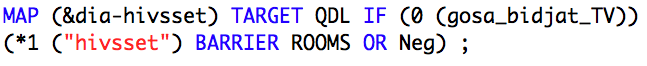
\includegraphics{img/hivsset_tag.png}} \\
\scalebox{0.55}[0.55]{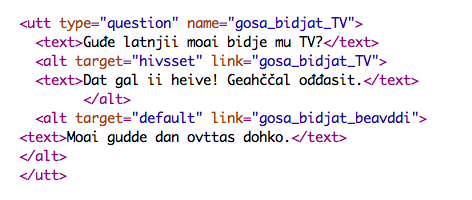
\includegraphics{img/gosabidjatTV.png}} \\
Question: "In which room should we place the TV?" \\
Alt. WC: "That is not a good idea. Make a new try." \\ 
Default: "We carry it there together." 
}


\frame{\frametitle{Navigating in the dialogue -- alternative branches} 
\scalebox{0.45}[0.45]{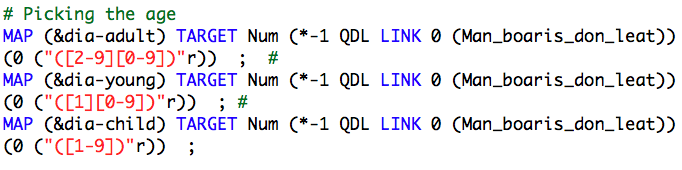
\includegraphics{img/pickingage_colours.png}} \\
\vspace{0.5cm} \pause
\scalebox{0.45}[0.45]{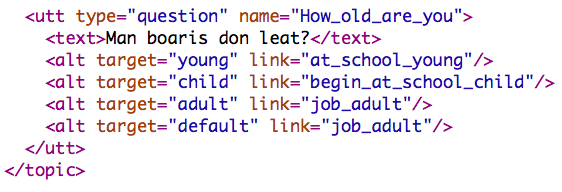
\includegraphics{img/age_branching.png}} \\
("How old are you?")
}

\section{4. Grammar feedback}


\frame{\frametitle{Disambiguation and assignment of grammar tag} 
\scalebox{0.3}[0.3]{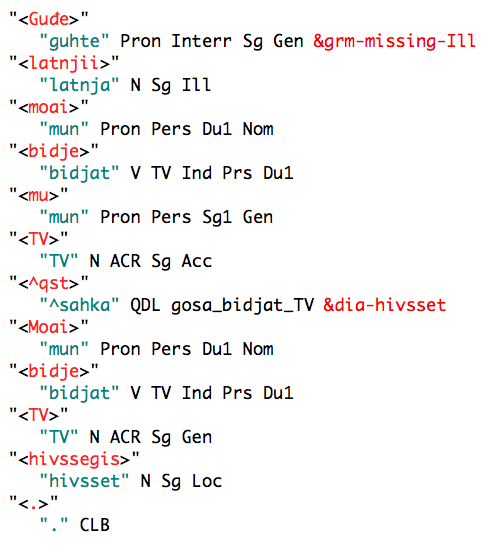
\includegraphics{img/hivssegisCGanal.png}} \\
\scalebox{0.35}[0.35]{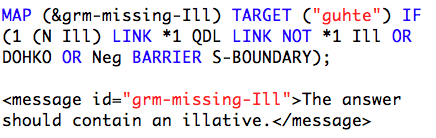
\includegraphics{img/missingIll.png}} \\
}

\section{5. Challenges}

%\frame{\frametitle{multi} 
%\scalebox{0.38}[0.38]{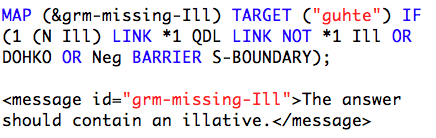
\includegraphics{img/missingIll.png}} \\
%}
\frame{\frametitle{Misspelling: non-existing word} 
\begin{itemize}
\item feedback: X is not in our lexicon. Could it be a typo?
\item What is your name?\\ we accept anything and pick the input $\rightarrow$ "Good morning, X."
\item Where do you live? \\
-- placename is misspelled \\
-- placename has not big initial letter \\ fst with placenames with small initial letter and Lowercase-error-tag which is removed so it remains if it is the only reading of the word form $\rightarrow$ Remember that placenames are written with capital letter.\\
-- placename is not in our lexicon $\rightarrow$ navigation to question: "I haven't heard about X. Is it a place?" -- default $\rightarrow$ next question. 
\end{itemize}
}

\frame{\frametitle{Misspellings: non-existing word} 
\begin{itemize}
\item One answer to this challenge is to utilize the North Sámi speller
\item Problem: it gives too many suggestions
\item Possible solution: Constraint the suggestion by CG rules
\end{itemize}
}


\frame{\frametitle{Misspellings: unintended word form} 
\begin{itemize}
\item Loc vs. px (\&grm-Px-shouldbe-Loc) $\rightarrow$ Do you mean locative? Remember consonant gradation. 
\item gfds
\item gfds
\item gfds
\item gfds
\end{itemize}
}

\frame{\frametitle{Misspellings: unintended lemma} 
\begin{itemize}
\item ConNeg -- bora vs. borat
\item gfds
\item gfds
\item gfds
\item gfds
\end{itemize}
}

%For misspellings that produce another word form of the same lemma, we have written rules that are based on the grammatical context. The real problem emerges when the spelling error gives rise to an unintended lemma. Then the challenge is to give a feedback according to what the student thinks she has written. In this case, feedback has to be tailored using the knowledge about the student’s interlanguage. We have created sets for typical unintended lemmata. Combined with contextual rules we can then give the user a good feedback due to the misspelling instead of the unintended lemma.
%
%E.g. if the student uses the Sg2 form of the main verb after the negative verb, instead of the correct ConNeg form, then the erroneous form can be a ConNeg form of a derivated verb, and the normal feedback will be: "You should answer with the same verb as in the question." The student will not understand this, because she thinks that the word form in the answer is an instance of the same verb. The solution was to generate all these forms of the verbs in the questions, make a set of them, and make a rule for in the right context, give the feedback: "The negative form is not correct." 


\frame{\frametitle{Answer with the same verb} 
\begin{itemize}
\item work verb
\item auxilary verbs
\item regular expression
\item  
\item  
\end{itemize}
}



\frame{\frametitle{Orthographic variation of words} 
\begin{itemize}
\item vuola:vuollaga vs. vuolla:vuola
\item dárbbašit vs. dárbbahit
\item gfds
\item gfds
\item gfds
\end{itemize}
}

\frame{\frametitle{Answer in the correct person} 
Vasta and Sahka different \\
QPN - question's person-number \\
APN - answer's person-number\\
\vspace{0.5cm}
\begin{tabular}[t]{ll|ll|ll}
QPN &APN &QPN &APN &QPN &APN \\
\hline
Sg1 &Sg2 &Du1 &Du2 &Pl1 &Pl2 \\
Sg2 &Sg1 &Du2 &Du1 &Pl2 &Pl1 \\
\hline
Sg3 &Sg3 &Du3 &Du3 &Pl3 &Pl3 \\
\hline
\end{tabular}
}

\frame{\frametitle{Meta comments} 
\begin{itemize}
\item Answering \textit{I-don't-know} is too simple. Try again.
\item Your answer must always contain a finite verb. Could there be a typo in the verbform?
\item You must use one of the words in the wordlist in the left margin.
\item You have not used the appropriate adjective. Try again.
\end{itemize}
}


\frame{\frametitle{What grammar errors we have rules for 1} 
Verbs and their arguments
\begin{itemize}
\item verbs: finite, infinite, correct tense, negative form
\item case of argument based upon the interrogative 
\item case of argument based upon valency
\item locative vs. illative based upon movement
\item subject/verbal agreement
\end{itemize}
}

\frame{\frametitle{What grammar errors we have rules for 2} 
Other
\begin{itemize}
\item agreement inside NP 
\item numeral expressions: case and number  
\item PP: case of noun, pp based upon the interrogative  
\item time expressions 
\item special adverbs  
\item particles according to word order 
\item comparision of adjectives
\end{itemize}
}



\section{6. Evaluation}

\frame{\frametitle{Evaluation 1}
\begin{table}
\begin{tabular}{|c|c|c|c|c|c|}
\hline
Morfa-S & Leksa & Sahka & Numra & Morfa-C & Vasta \\
41\% & 27\% & 13\% & 12\% & 5\% & 2\% \\
\hline
\end{tabular}
\end{table}
}

\frame{\frametitle{Evaluation 2}
\begin{table}
\begin{tabular}{|l|c|c|c|}
\hline 
\textbf{Rule type}  & \textbf{correct} & \textbf{wrong}   & \textbf{corr. \% }  \\
\hline 
wrong tense         & 7     & 0     & 100,0     \\ 
wrong V after neg   & 3     & 0     & 100,0     \\ 
no infinite V       & 1     & 0     & 100,0     \\ 
\hline 
orth. error         & 44    & 2     & 95,7      \\
wrong case for V-arg  & 26    & 4     & 86,7      \\
no finite verb        & 19    & 4     &  82,6 \\
\hline 
wrong S-V agreement   & 17    & 8     & 68,0 \\
wrong V choice        & 7     & 4     & 63,6 \\
\hline 
wrong word            & 4     & 4     & 50,0 \\
wrong case after Num  & 1     & 1     & 50,0 \\
\hline
\end{tabular}
\end{table}
}

\frame{\frametitle{Evaluation 3}
Which rules are not in use? Why? \\
\begin{itemize}
\item agreement inside NP 
\item PP: case of noun, pp based of the interrogative  
\item time expressions 
\item particles according to word order 
\end{itemize}

}


\frame{\frametitle{An alternative to free input: the German e-tutor} 
\scalebox{0.45}[0.45]{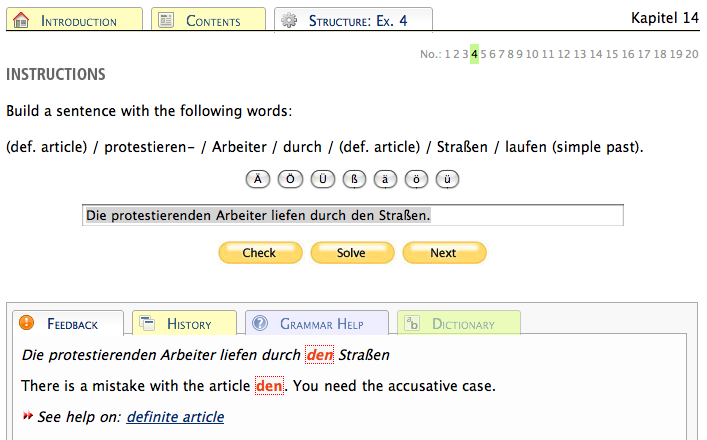
\includegraphics{img/e-tutor.png}} \\
}

\frame{\frametitle{Evaluation 4: Precision and recall}
\begin{table}%[htdp]
%\caption{default}
%\begin{center}
\begin{tabular}{|l|r|r|r|r||r|r|r|r|r|}
\hline
Error type	& tp		& fp		& tn		& fn	& prec	 & rec.	& acc.	& F-ms. \\
\hline
Gramm. err. & 743 & 276 & 783 & 7 & 0,73 & 0,99 & 0,84 & 0,84   \\
Sem. err.   & 942 & 77 & 777 & 13 & 0,92 & 0,99 & 0,95 & 0,95   \\
Orth. err   & 1019 & 0 & 790 & 0 & 1 & 1 & 1 & 1			    \\
Other err.  & 839 & 180 & 765 & 25 & 0,82 & 0,97 & 0,89 & 0,89  \\
\hline
Average & 3543   & 533 & 3115  & 45  & 0,87 & 0,99 & 0,92 & 0,92    \\
\hline
\end{tabular}
%\end{center}
%\label{default}
\end{table}%

The high recall compared to the somewhat lower precision indicates that the system is a bit too critical towards the students:
\begin{itemize}
\item{It almost never lets through a (targeted) mistake, with the price of flagging some correct answers as errors.}
\end{itemize}
}


\section{7. Future perspectives}
\frame{\frametitle{Future perspectives}
How to improve the system? \\
\begin{itemize}
\item speller for misspellings 
\item grammartasks a la \textit{e-tutor}?
\item Vasta: options based on pragmatics, not grammar
\item Vasta: option for training complex NP, time expressions and so on
\end{itemize}

}




\section{8. Conclusion}
\frame{\frametitle{Conclusion}

\begin{itemize}
\item By using a sloppy version of the syntactical analyser for North Sámi, combined with a set of error-detection rules, we have been able to build a flexible CALL resource. \\ \pause
\vspace{0.5cm}
\item The present project has shown that CG is well fit for making pedagogical dialogue systems.\\ \pause
\vspace{0.5cm}
\item The program suite is something quite new among pedagogical programs for Sámi, and indeed its dialogue and open QA-programs are quite rare within the field of parser-based CALL.
\end{itemize}
}

\frame{\frametitle{Acknowledgments} 
Thanks to the faculty of Humanities at the University of Tromsø, and the Sámi Parliament in Norway, for funding the project.
} 

%\frame{\frametitle{References} 
%\scalebox{0.32}[0.32]{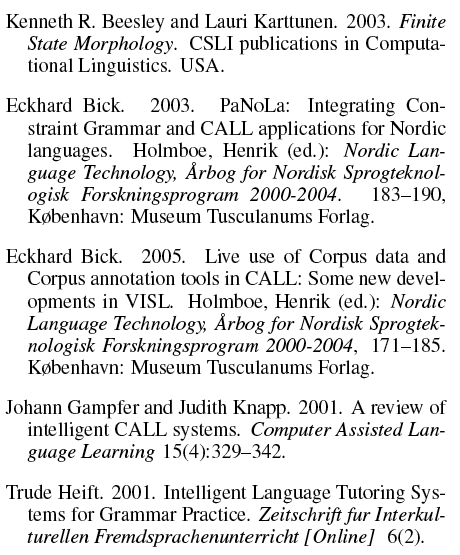
\includegraphics{img/ref1.png}}
%\scalebox{0.32}[0.32]{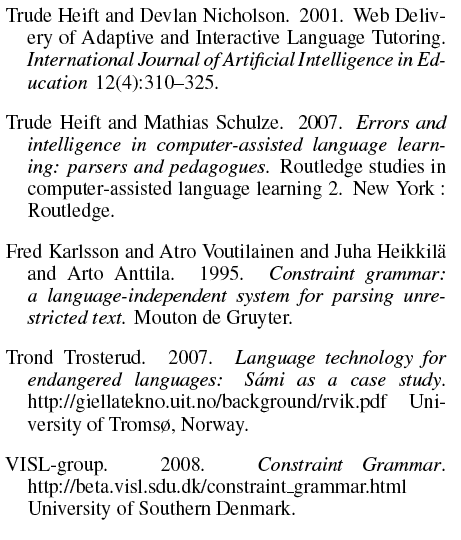
\includegraphics{img/ref2.png}}




\frame{\frametitle{Questions?} 
} 



\end{document}

